\documentclass[main]{subfiles}

\begin{document}
\begin{lect}
	\subsection{Дробно-линейное  отображение.  Круговое  свойство.  Другие  св-ва (б/д)}

	\begin{Definition}
		\[\sin z = \dfrac{e^iz - e^{-iz}}{zi}\]
		\[\sin z = -i \sh(iz)\]
		Период $f(z) = \sin z \q T = 2\pi k,\q k \in \Z$\\
		$g(z) = \sh z$ - период $2 \pi i$
		\[\cos z = \dfrac{e^{iz} + e^{-iz}}{z} = \ch(iz)\]
		\[\ch z = \dfrac{e^z + e^{-z}}{z}\]
	\end{Definition}

	\begin{Definition} [функция Жуковского]
		\[\text{Ж}(z) = \frac{1}{2} (z + \frac{1}{z})\]
		\[T = \{z : \abs{z} = 1\}\]
		\begin{figure}[H]
			\centering
			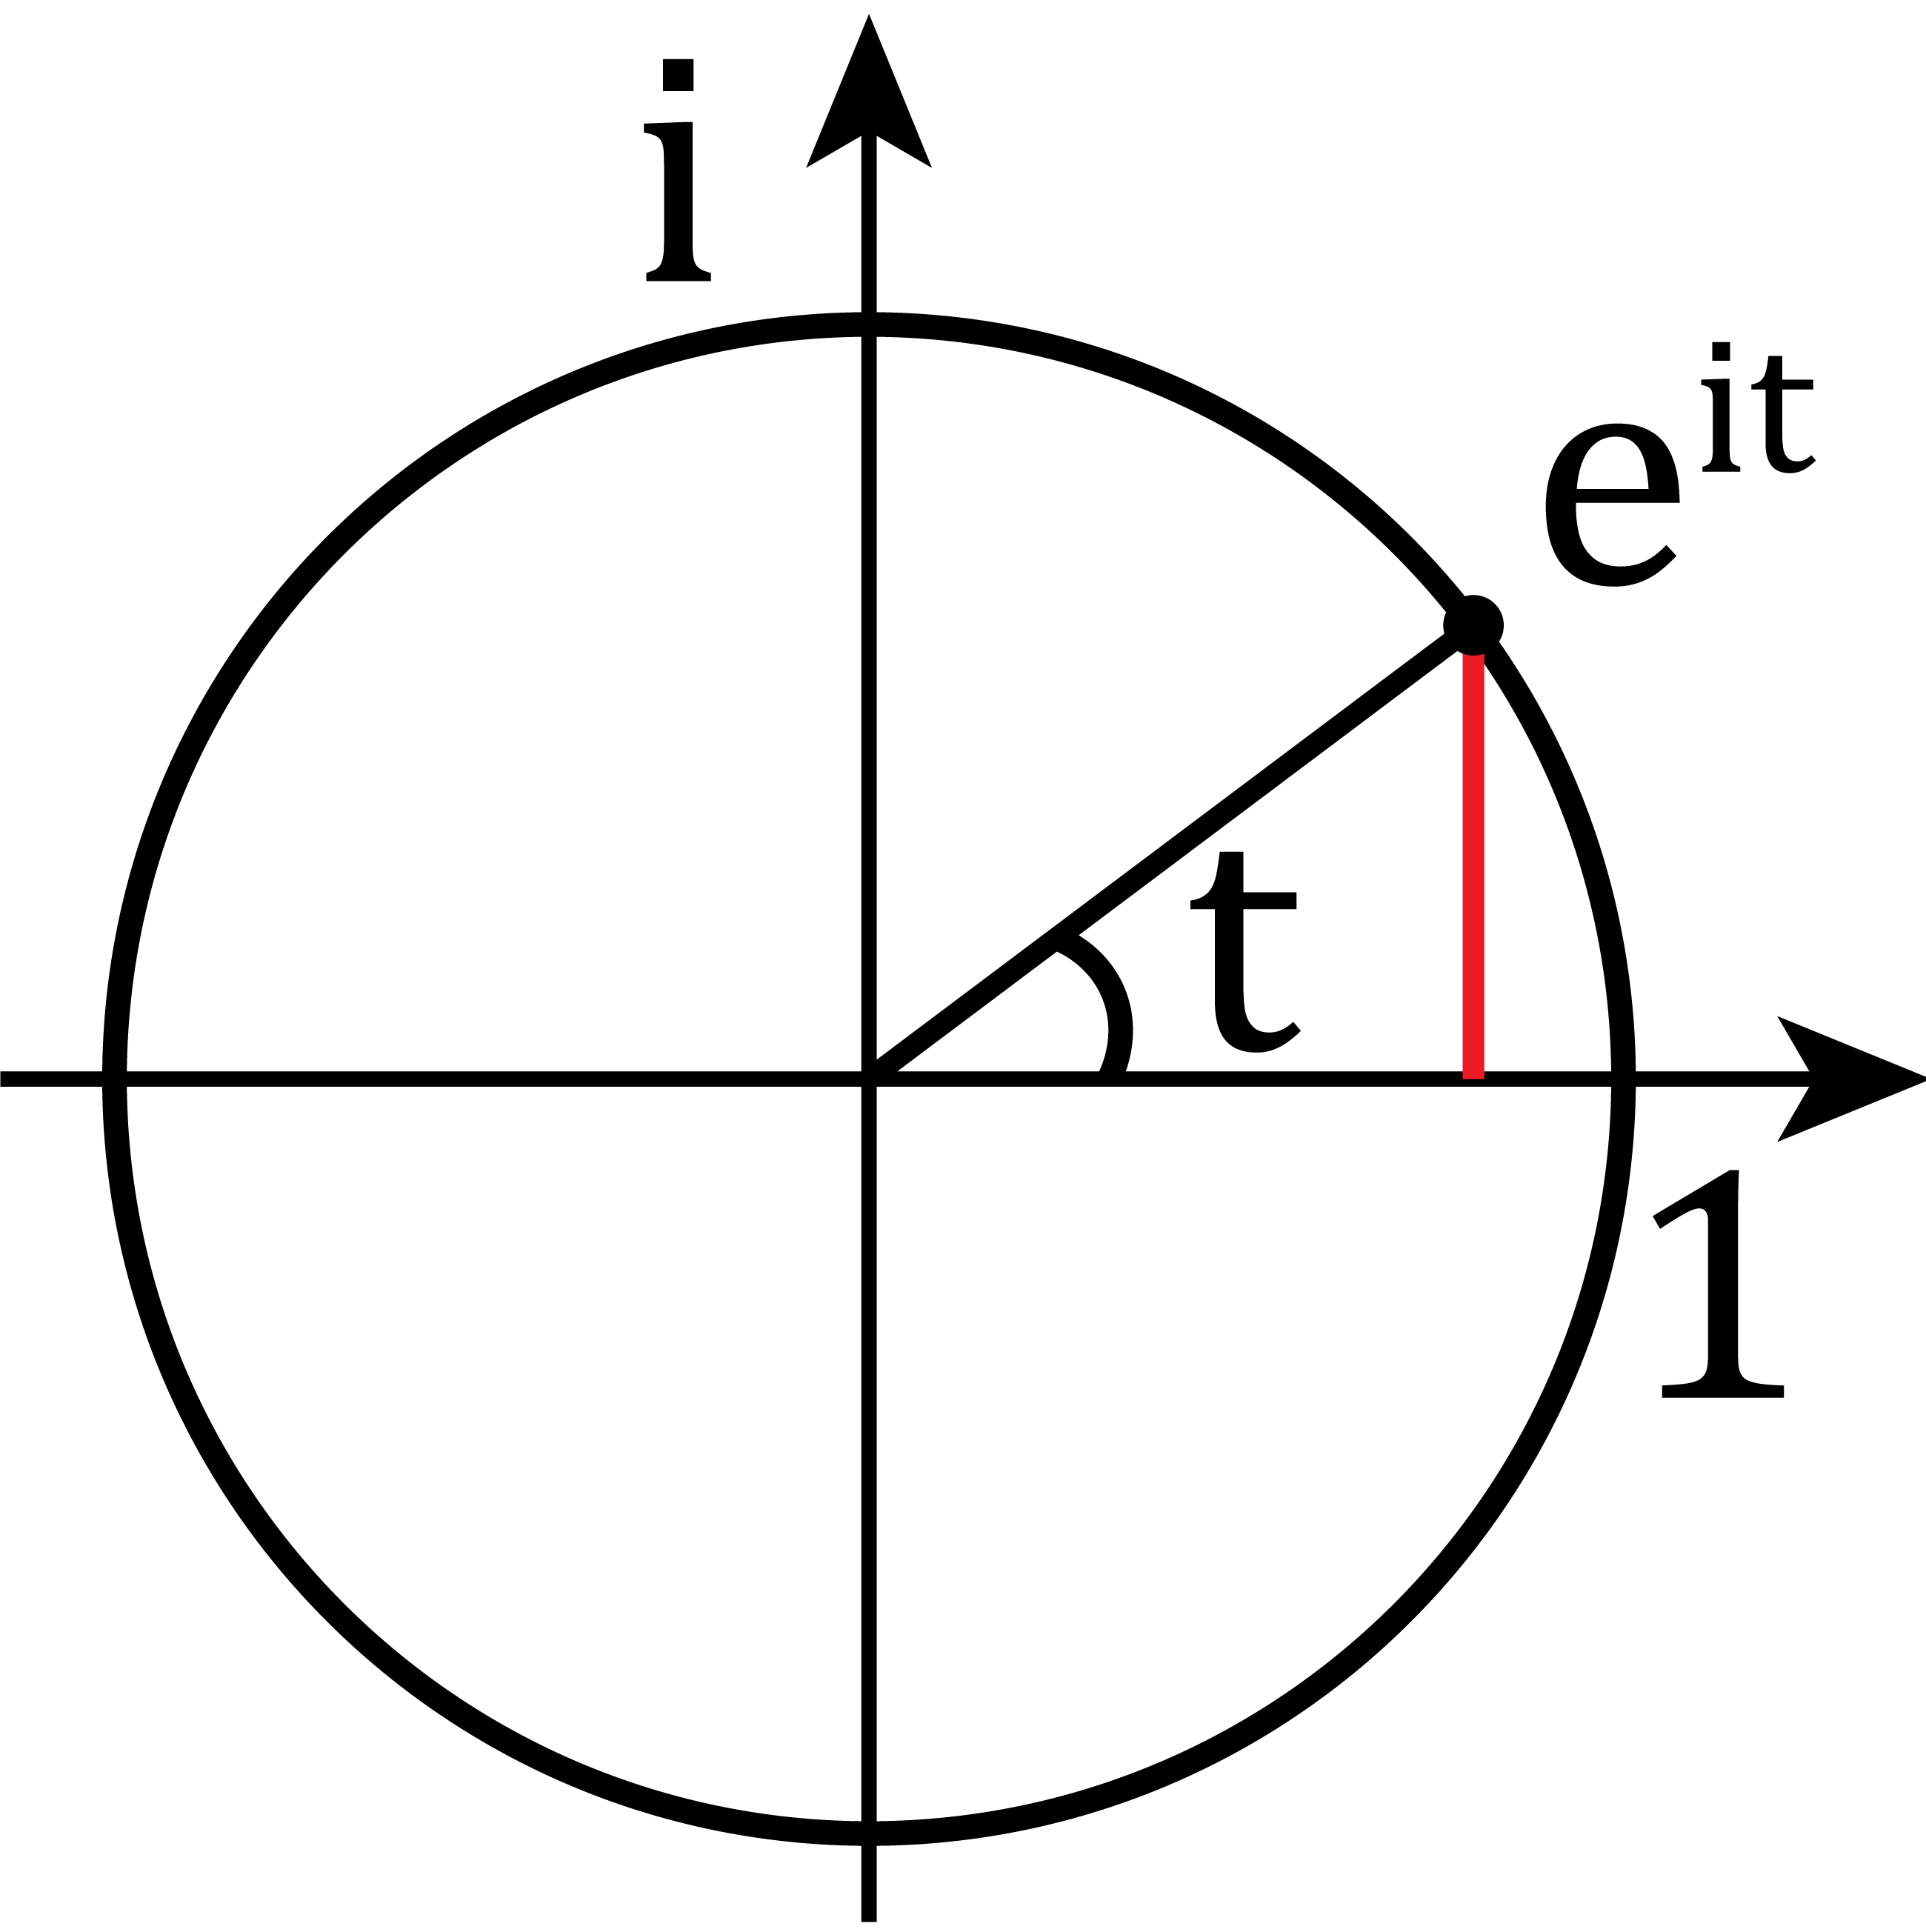
\includegraphics[width=3.5cm]{9_1}
		\end{figure}
		\[z = e^{it} = \cos t + i \sin t \]
		\[- \pi \leq t \leq \pi\]
		\[\text{Ж}(e^{it}) = \frac{1}{2} (e^{it} + e^{-it} ) = \cos t = \text{Ж}(e^{-it})\]
		\[\text{Ж}(T) = [-1, 1] \text{не вз-одн} \] %?what не вз-одн?
		Прообраз $\forall a \in (-1, 1) $ сост. из двух т.
		\[rT = \{r e^{it}, -\pi \leq t \leq \pi\}\]
		\[0 < r < 1\]
		\[\text{Ж}(r e^{it}) = \frac{1}{2}(r e^{it} + \frac{1}{r} e^{-it} ) =
			\frac{1}{2} (r + \frac{1}{r}) \cos t + i \frac{1}{2} (r - \frac{1}{r}) \sin t\]
		\begin{figure}[H]
			\centering
			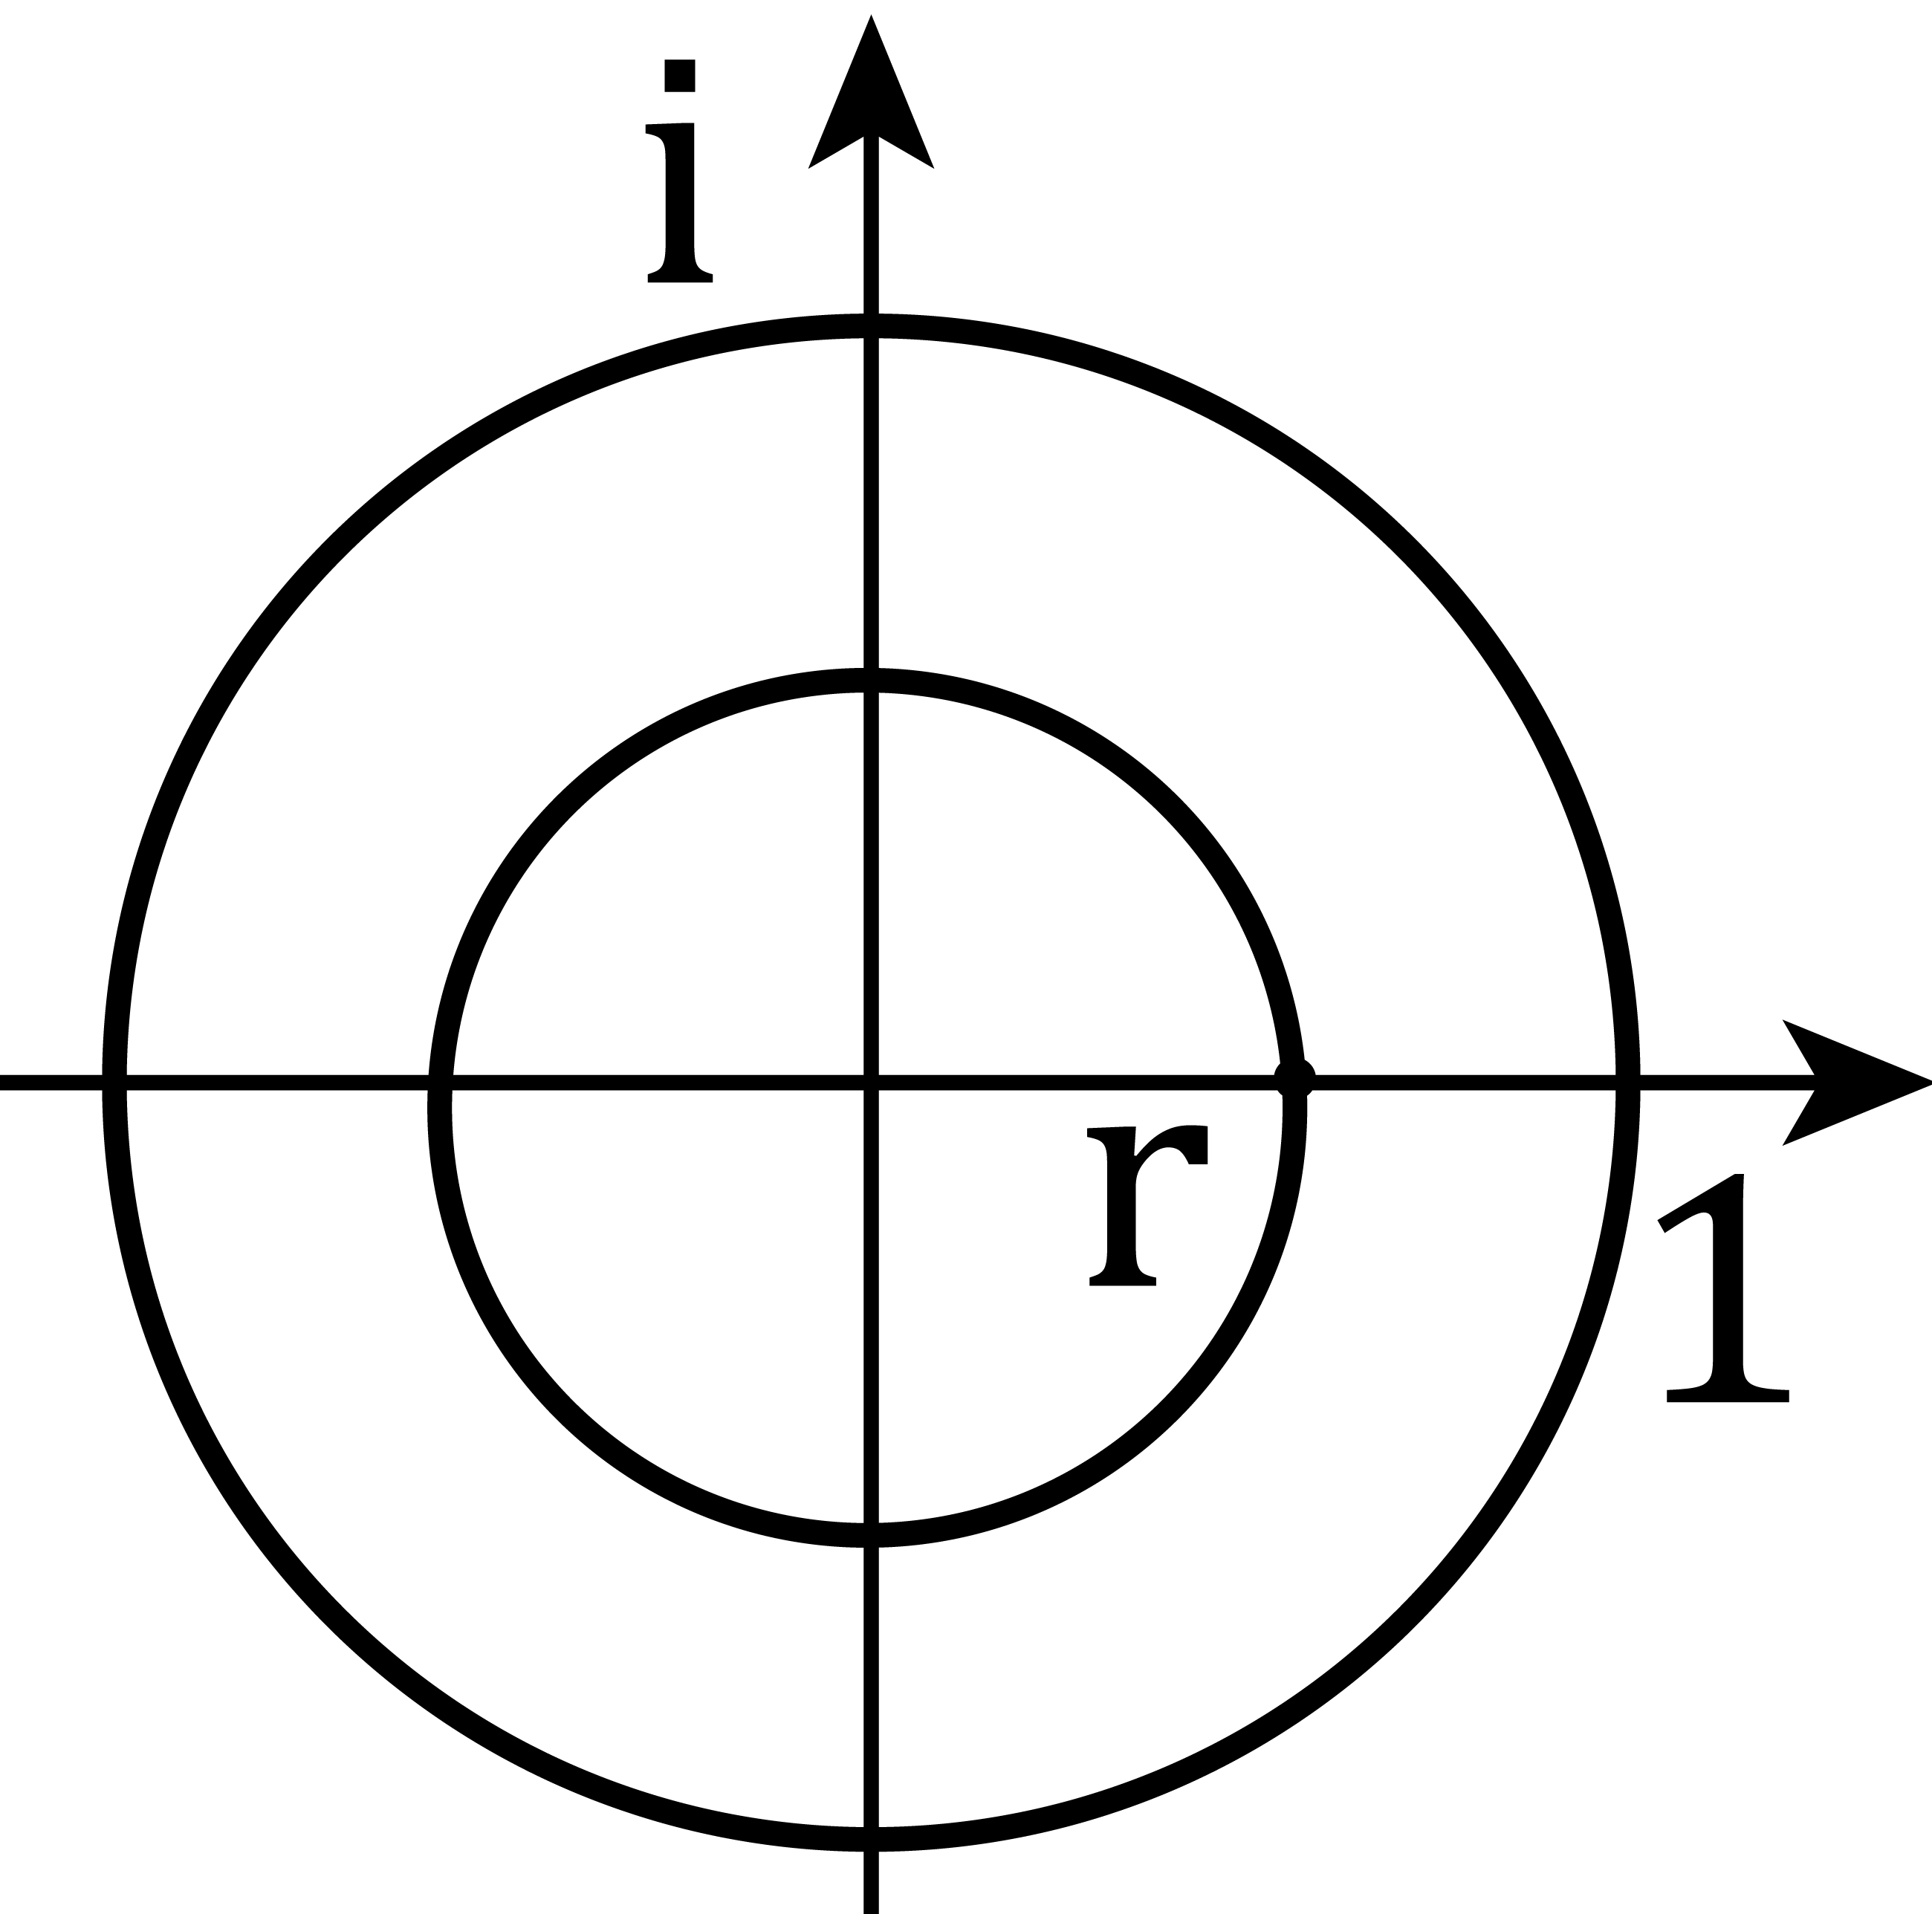
\includegraphics[width=3.5cm]{9_2}
		\end{figure}
		\[\begin{cases}
				\real \text{Ж} (r e^{it} ) = \frac{1}{2} (r + \frac{1}{r}) \cos t \\
				\im \text{Ж} (r e^{it} ) = \frac{1}{2}(r - \frac{1}{r}) \sin t
			\end{cases} \text{ - пар. ур. эллипса с полуосями}\]
		\[a = \frac{1}{2} (r + \frac{1}{r}) \geq 1\]
		\[-b = \frac{1}{2} (r - \frac{1}{r})\]
		\[b = \frac{1}{2}(\frac{1}{r} - r)\]
		\[-\pi \leq t \leq \pi\]
		\begin{figure}[H]
			\centering
			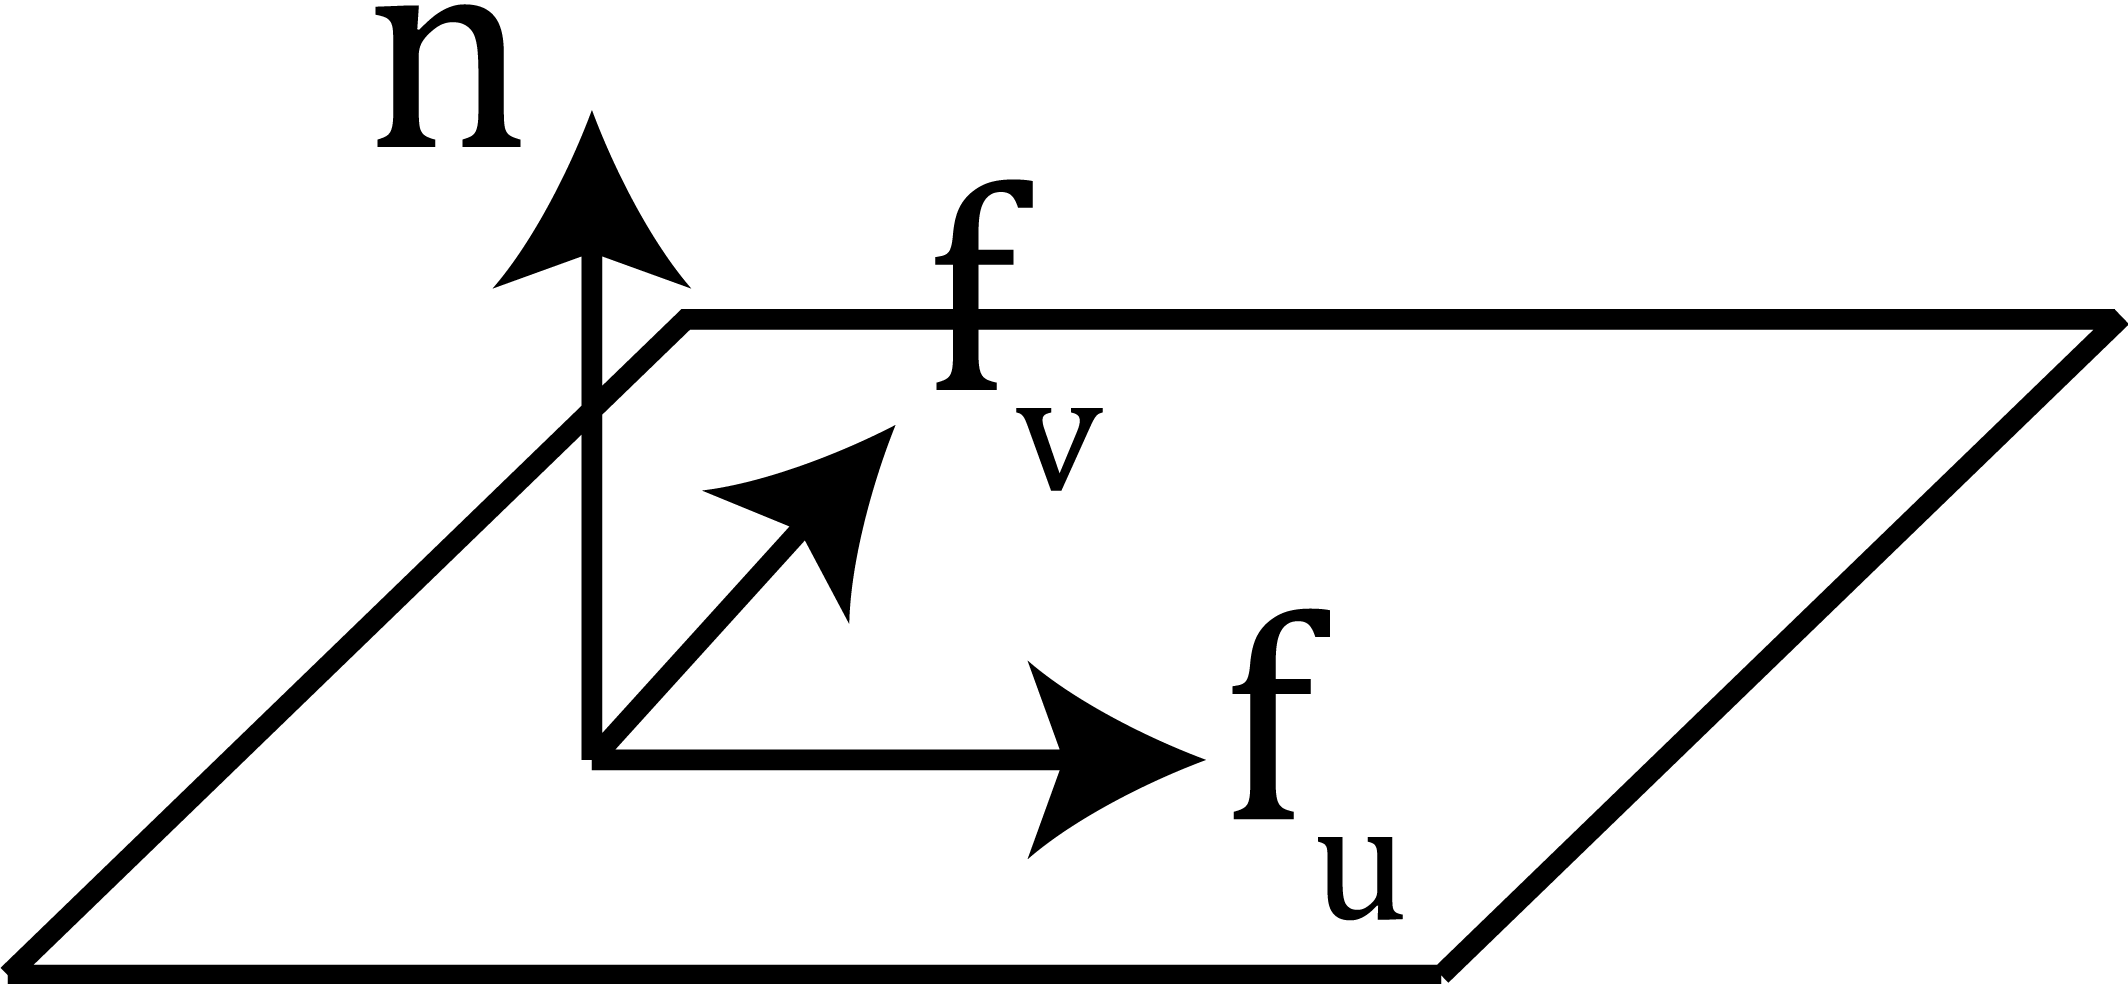
\includegraphics[width=7cm]{9_3}
		\end{figure}
		\[R > 1 \qq \text{Ж} (R e^{it} ) = \frac{1}{2} (\us{\geq 1}{R + \frac{1}{R}})\cos t + i \frac{1}{2}
			(\us{\geq 0}{R - \frac{1}{R}}) \sin t\]
		\[\cos z = \frac{e^{iz} + e^{-iz}}{z} = \text{Ж}(e^{iz} )\]
		\begin{figure}[H]
			\centering
			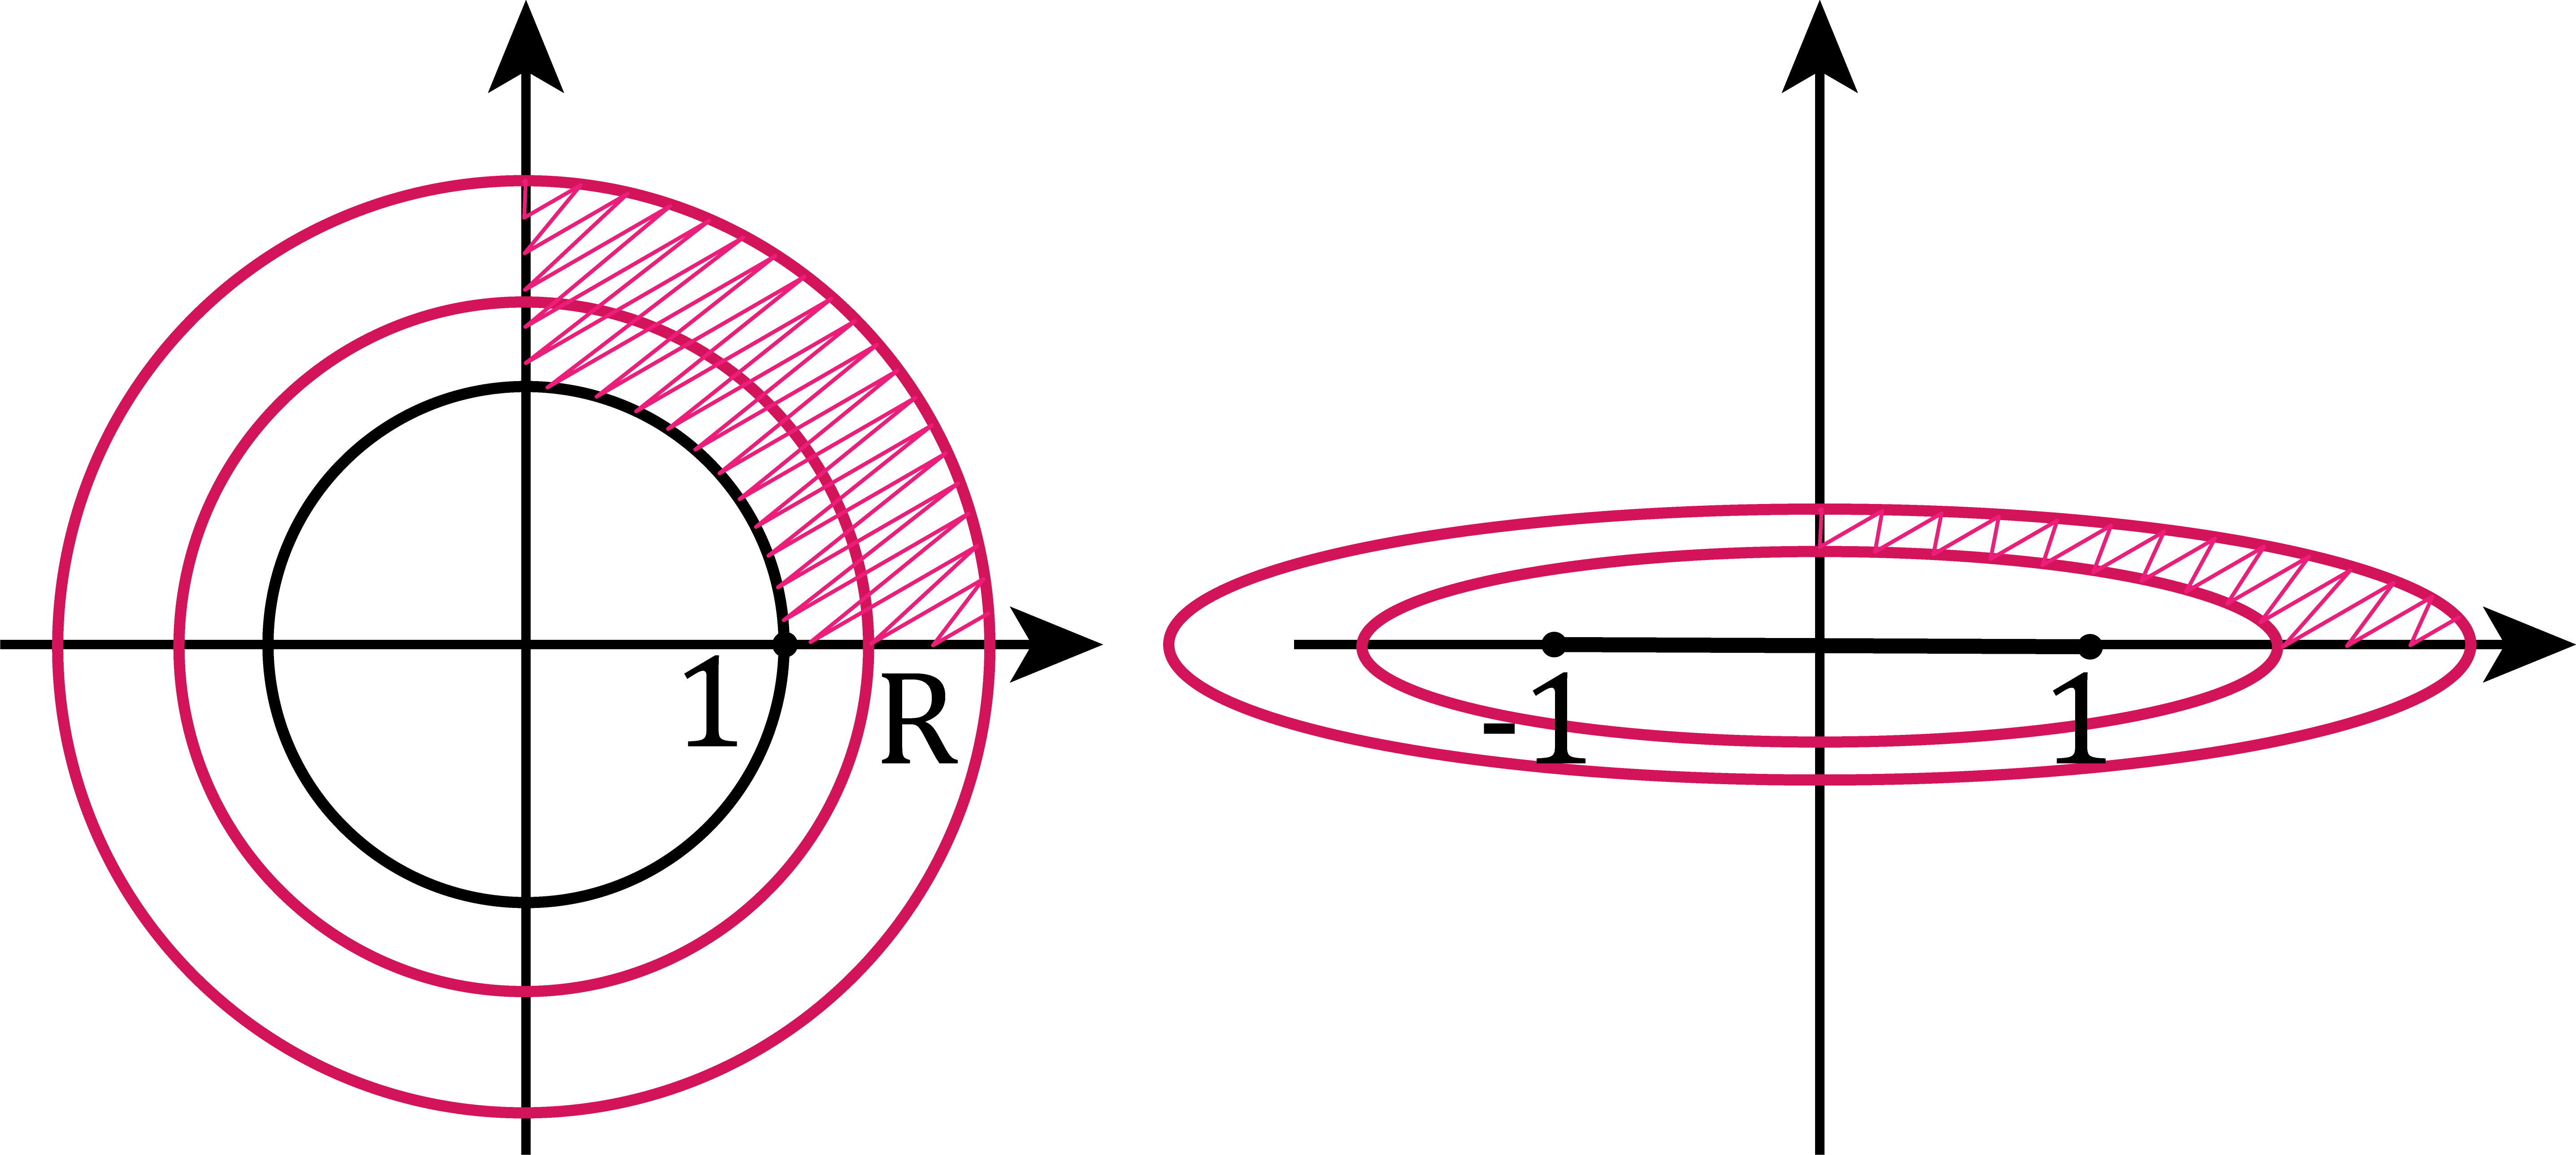
\includegraphics[width=7cm]{9_4}
		\end{figure}
	\end{Definition}

	\begin{Definition} [аргумент комплексного числа]
		\[z = x + iy; \q \abs{z} = \sqrt{x^2 + y^2}\]
		\begin{figure}[H]
			\centering
			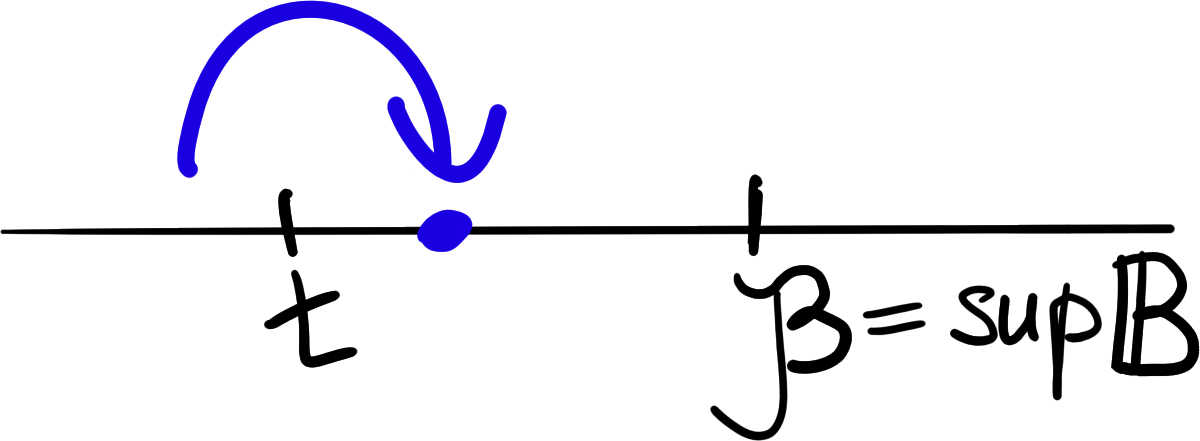
\includegraphics[width=3cm]{9_5}
		\end{figure}
		\[z \to \abs{z}; \text{ угол } \varphi \qq z = \abs{z} (\cos \varphi + i \sin \varphi)\]
		Подходят все углы $\varphi + 2 \pi k, \q k \in \Z$
		\[\text{Arg} z = \{\varphi + 2\pi k, \q k \in \Z\} \text{ --- полное знач. арг.}\]
		Отображение $\text{Arg} : \CC \to $\\
		$\forall z \in \CC $ сопоставляет множество
	\end{Definition}

	\begin{Definition} [непрерывная ветвь аргемнта]
		\[\text{Ф-я } \alpha : \Omega \to \R \qq \Omega \subset \CC\]
		Называется непр. ветвью аргумента $z$, если
		\[\alpha \in C(\Omega) \text{ и } \forall z \in \Omega \q \alpha(z) \in \text{ Arg} z\]
	\end{Definition}

	\begin{Example}
		\[\Omega = \{\abs{z} < 1\} \text{ здесь нельзя определить однозн. ветвь аргумента}\]
		\begin{figure}[H]
			\centering
			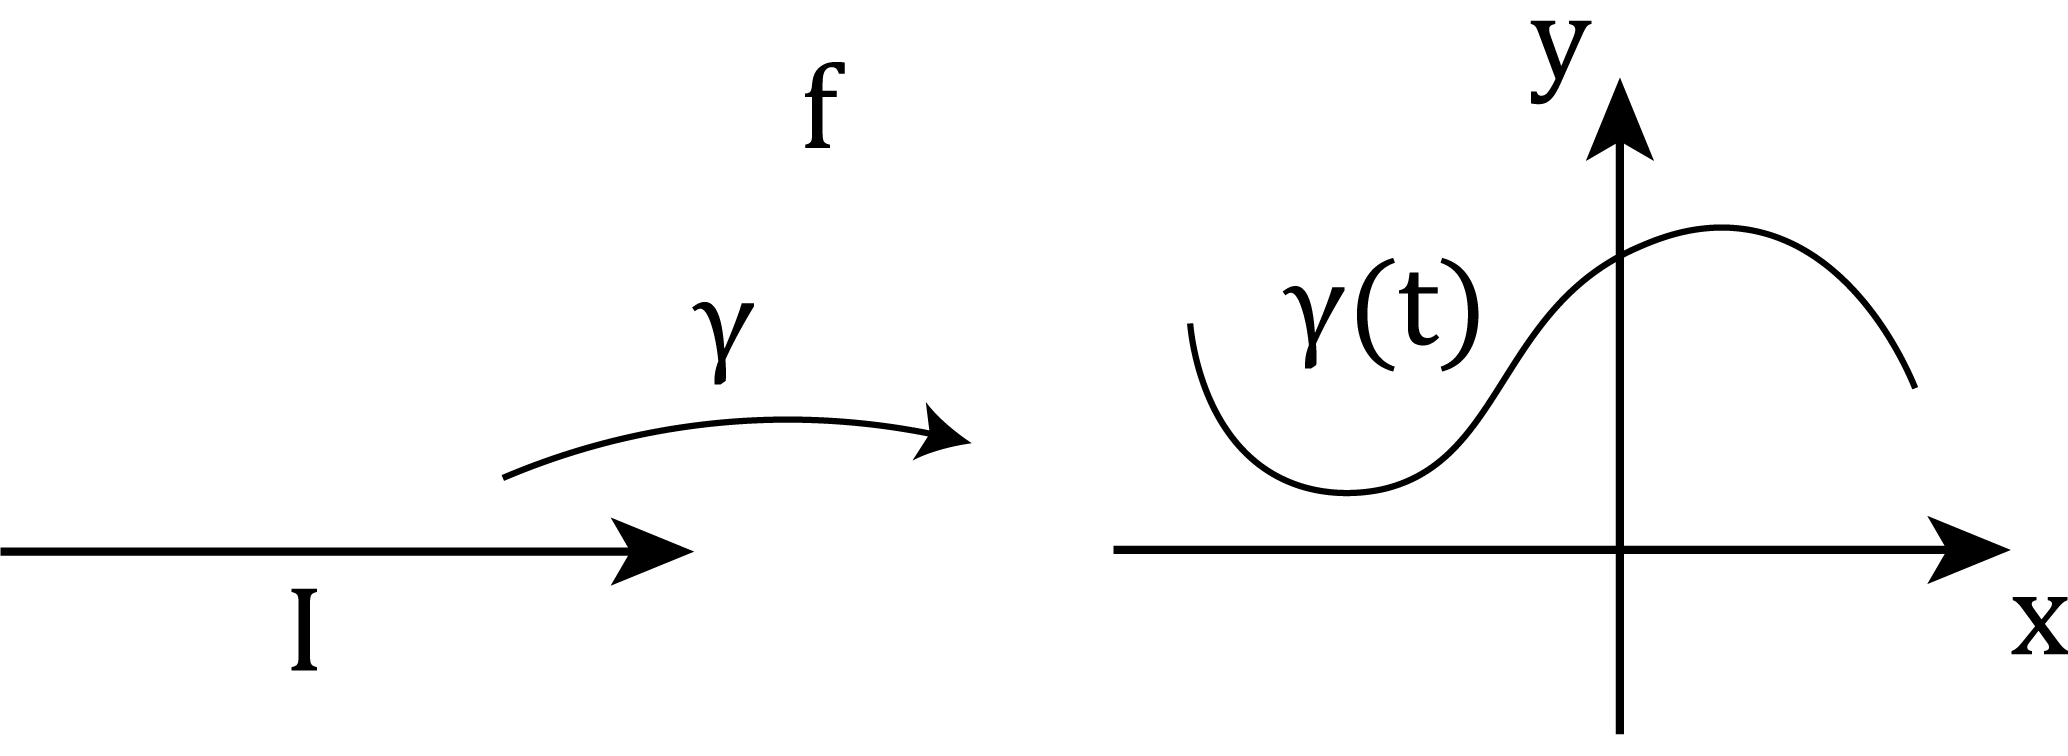
\includegraphics[width=3.5cm]{9_6}
		\end{figure}
		\[\Omega = \CC \setminus \{z = x;\q x \in (- \infty, 0]\}\]
		Главное значение аргумента
		\[\begin{cases}
				\text{arg} (z) \in \text{Arg}(z) \\
				\text{arg} (z) \in (-\pi, \pi)
			\end{cases}\]
		\[z = x < 0 \qq \text{arg}(z) = \pi\]
		\[\text{Arg } z = \{\text{arg } z + 2 \pi k, k \in \Z\}\]
		\[\text{Arg } z = \text{arg } z + 2 \pi k\]
	\end{Example}

	\begin{Example} [некоторые многозначные функции]
		\[w^n = z, \q n \in \N\]
		Уравнение имеет $n$ решений
		\[w = \abs{w} \cdot e^{i \text{Arg } w}  \q z = \abs{z} \cdot e ^{i \text{Arg }z} \]
		\[\begin{cases}
				\abs{w}^n = \abs{z} \\
				n \text{Arg } w = \text{Arg } z
			\end{cases}\]
		\[\abs{w} = \us{\R}{\sqrt[n]{\abs{z}}} \qq \us{\R}{\sqrt[n]{x}} = x^{\frac{1}{n}}  \q x \in \R\]
		\[n \text{Arg } w = \text{arg } z + 2 \pi k, \q k \in \Z\]
		\[\text{Arg } w = \left\{\frac{\text{arg } z}{n} + \frac{2 \pi k }{n}, \q k \in \Z\right\}\]
		\[w = \us{\CC}{\sqrt[n]{z}} = \us{\R}{\sqrt[n]{\abs{z}}} \cdot e^{i (\frac{\text{arg } z}{n} +
					\frac{2 \pi k }{n})} \]
		\[\forall z \in \CC \setminus \{0\}\]
		\[\sqrt[n]{z} \text{ принимает } n \text{ разл. знач.}\]
	\end{Example}

	\begin{Definition} [комплексный логарифм]
		\[e^w = z\]
		\[w = u + iv\]
		\[e^{u + iv} = e^u \cdot e^{iv} = \abs{z} \cdot e^{i \text{Arg z}} \]
		\[\begin{cases}
				e^u = \abs{z} \\
				v = \text{Arg } z
			\end{cases} \qq \begin{cases}
				u = \us{\R}{\ln} \abs{z} \\
				v = \text{arg } z + 2 \pi k
			\end{cases}\]
		\[w = \us{\R}{\ln} \abs{z} + i (\text{arg } z + 2\pi k) = \us{\R}{\ln } \abs{z} + i \text{Arg } z\]
		\[\ln z = \us{\R}{\ln}\abs{z} + i \text{arg } z\]
		Если $x > 0$, то arg $x$ = 0
		\[\ln x = \us{\R}{\ln} x + i0\]
		\[\text{Ln } z = \ln \abs{z} + i \text{Arg } z\]
		\[\text{Ln } z = \ln z + 2 \pi k i\]

		\[a, b \in \CC \q a \neq 0\]
		\[a^b = e ^ {(\text{Ln a})b}\]
		\[i^i = e^{(\text{Ln } i)i} \]
		\[\text{Ln } i = \ln \abs{i} + i \text{Arg } i = 0 + i (\frac{\pi}{2} + 2 \pi k)\]
	\end{Definition}

	\begin{Definition} [обратные тригонометрические функции]
		\[\cos w = z\]
		\[e^{iw} + e^{-iw} = 2z\]
		\[e^{iw} = t \qq t^2 - 2t \cdot z + 1 = 0\]
		\[t = z + \sqrt{z^2 - 1} = e^{iw} \]
		\[iw = \text{Ln } (z + \sqrt{z^2 - 1})\]
		\[\arccos z = -i \cdot\text{Ln } (z = \sqrt{z^2 - 1})  \os{*}{=}\]
		\[z + \sqrt{z^2 - 1} = \frac{1}{z - \sqrt{z^2  - 1}}\]
		\[\os{*}{=} i \text{Ln } (z - \sqrt{z^2 - 1})\]
	\end{Definition}

	\begin{Example}
		\[\text{Решим уравнение } \sin z = i\]
		\[e^{iz} - e^{-iz} = 2i^2 = -2  \]
		\[e^{iz}  = t\]
		\[t^2 + 2t - 1 = 0\]
		\[t = -1 + \us{\CC}{\sqrt{1 + 1}} = \pm \us{\R}{\sqrt{2}} - 1 \qq \sqrt{2} - 1 = \frac{1}{\sqrt{2} + 1}\]
		\[iz = \text{Ln} (\pm \sqrt{2} - 1)\]
		\[\bigg[\begin{align}
				 & iz = \ln(\sqrt{2} - 1) + i (2 \pi k)          \\
				 & iz = \ln(-\sqrt{2} - 1) + i (\pi + 2 \pi k) =
			\end{align}\]
		\[ = \ln(- \frac{1}{\sqrt{2} - 1}) + i (\pi + 2\pi k) = -\ln(\sqrt{2} - 1) + i 2 \pi k\]
	\end{Example}

	\subsection{Комплексное дифференцирование. Условия Коши-Римана}
	\begin{Definition}
		\[\Omega \subset \CC \qq \Omega \text{ --- область, если:}\]
		\begin{enumerate}
			\item $\Omega$ --- откр.
			\item $\forall a, b \in \Omega $ можно соед. ломанной ($\Omega$ --- связно)
		\end{enumerate}
	\end{Definition}

	\begin{Definition}
		\[f : \Omega \to \CC \qq z_0 \in \CC\]
		\[f \text{ --- ди-ма } (\CC \text{ --- диф-ма}) \text{ в т. } z_0\text{, если:}\]
		\[\exists A \in \CC : \q f(z) = f(z_0) + A(z - z_0) + o(\abs{z - z_0}) \qq z \to z_0\]
		\[A = \us{\text{произв. } f}{f'(z_0)} = \lim_{z \to z_0} \frac{f(z) - f(z_0)}{z - z_0} =
			\lim_{\Delta z \to 0} \frac{f(z_0 + \Delta z) - f(z_0)}{\Delta z} \]
		\[z - z_0 = \Delta z\]
		Предел не зависит от того, как $\Delta z \to 0$
	\end{Definition}

	\begin{Example} [1]
		\[f(z) = \overline{z} \qq z_0 = 0\]
		\[f'(0) =? \lim_{\Delta z \to 0} \frac{\overline{\Delta z} - 0}{\Delta z} =
			\lim_{\Delta \to 0} \frac{\Delta x - i \Delta y}{\Delta x + i \Delta y} \]
		Если $\Delta z = \Delta x \to 0$, то $\displaystyle \lim_{\Delta z \to 0} \frac{\overline{\Delta z}}
			{\Delta z} = 1 $ \\
		Если $\Delta z = i\Delta y \to 0$, то $\displaystyle \lim_{\Delta z \to 0} \frac{\overline{\Delta z}}
			{\Delta z} = -1 $
	\end{Example}

	\begin{Example} [2]
		\[f(z) = z^n, \q n \in \N\]
		\[f'(z_0) = \lim_{\Delta z \to 0} \frac{(z_0 + \Delta z)^n - z^n}{\Delta z} = \]
		\[ = \lim_{\Delta z \to 0} \frac{z_0^n + n \Delta z z_0^{n - 1} + C^2_n \Delta z^2 z_0^{n - 2} + ...+
			\Delta z^n - z_0^n}{\Delta z} = n \cdot z_0^{n - 1}  \]
	\end{Example}

	\begin{theorem} [основные правила диф-я]
		\begin{enumerate}
			\item $(f + g) = f' + g'$
			\item $(\const \cdot f)' = \const \cdot f'$
			\item $(f \cdot g)' = f'g + fg'$
			\item $[f(g(z))]' = f'(g(z)) \cdot g'(z)$
		\end{enumerate}
	\end{theorem}

	\begin{utv}
		Если $f$ --- диф-ма в т. $z_0$, то она непр. в $z_0$
	\end{utv}

	\begin{Proof}
		\[f(z) - f(z_0) = f'(z_0) \cdot (z - z_0) + o(\abs{z - z_0}) \q z \to z_0 \Ra\]
		\[\Ra f(z) \to f(z_0) \q z \to z_0\]
	\end{Proof}

	\begin{Definition}
		\[\us{\text{Область}}{\Omega \subset \CC} \qq z = x + iy \in \CC \rla (x, y) \in \R\]
		\[f : \Omega \to \CC \qq f(z) = u(x, y) + iv(x, y)\]
		\[z \to (x, y) \to u(x, y) = \real f (x + iy)\]
		\[\q\q\q\q\q\q v(x, y) = \im f(x + iy)\] % костыль хы
		\[u : \Omega \to \R\]
		\[v : \Omega \to \R\]
		\[\begin{pmatrix}
				u \\
				v
			\end{pmatrix} : \Omega \to \R^2\]
	\end{Definition}

	\subsection{Комплексное дифференцирование. Условия Коши-Римана}

	\begin{Theorem} [условие Коши-Римана (Эйлера-Даламбера)]
		\[\Omega \subset \CC \text{ - область}\]
		\[f : \Omega \to \CC \qq f(x + iy) = u(x, y) + iv(x, y)\]
		Следующие условия равносильны
		\begin{enumerate}
			\item $f$ --- диф-ма $(\CC)$ в т. $z_0 \in \Omega$
			\item $u, v$ --- диф-мы в т. $(x_0, y_0)\q z_0 = x_0 + i y_0$
		\end{enumerate}

		\[\begin{cases}
				\frac{\partial u}{\partial x} (x_0, y_0) = \frac{\partial v}{\partial y}(x_0, y_0) \\
				\frac{\partial u}{\partial y} (x_0, y_0) = -\frac{\partial v}{\partial x}(x_0, y_0)
			\end{cases}\]
	\end{Theorem}

	\begin{Proof}
		\[(1 \Ra 2) \q \text{ предпол., что } f \text{ --- диф-ма в т. } z_0 \qq \Delta z = z - z_0\]
		\[f(z) = f(z_0) + f'(z_0) \cdot \Delta z + o(\abs{\Delta z}) \qq f(z) = u + iv\]
		\[f'(z_0) = A = a + ib \qq z = \Delta x + i\Delta y\]
		\[o(\abs{\Delta z}) = h(\Delta z) \cdot \abs{\Delta z}
			= (\alpha(\Delta x, \Delta y) + i \beta (\Delta x, \Delta y)) \abs{\Delta z}\]
		\begin{multline*}
			u(x, y) + iv(x, y) = u(x_0, y_0) + iv(x_0, y_0) + (a + ib)(\Delta x + i\Delta y) + \\
			+ (\alpha(\Delta x, \Delta y) + i\beta(\delta x, \delta y)) \abs{\Delta z}
		\end{multline*}
		\begin{multline*}
			u(x, y) = u(x_0, y_0) + a \cdot \Delta x - b \Delta y + \alpha(\Delta x, \Delta y) \sqrt{\Delta x^2 +
				\Delta y^2}
		\end{multline*}
		\begin{multline*}
			u(x, y) = v(x_0, y_0) + b \cdot \Delta x - a \Delta y + \beta(\Delta x, \Delta y) \sqrt{\Delta x^2 +
				\Delta y^2}
		\end{multline*}
		\[\alpha, \beta \to 0 \qq \sqrt{\Delta x^2 + \Delta y^2} \to 0\]
		т.о $u, v $ - дифф-мы в т. $(x_0, y_0)$
		\[\frac{\partial u}{\partial x}(x_0, y_0) = a \q \frac{\partial u}{\partial y}(x_0, y_0) = -b\]
		\[\frac{\partial v}{\partial x}(x_0, y_0) = v \q \frac{\partial v}{\partial y}(x_0, y_0) = a\]
		\[\Ra \begin{cases}
				\frac{\partial u}{\partial x}(x_0, y_0) =   & \frac{\partial v}{\partial y}(x_0, y_0) \\
				\frac{\partial u}{\partial y}(x_0, y_0) = - & \frac{\partial v}{\partial x}(x_0, y_0)
			\end{cases}\]
		Условие К-Р, Э-Д

		\[(2 \Ra 1) \q \text{Пусть } u, v : \Omega \to \R \text{ диф-мы } (x_0, y_0)\]
		\[u(x, y) = u(x_0, y_0) + \frac{\partial u}{\partial x}\Delta x + \frac{\partial u}{\partial y}(x_0, y_0)
			\Delta y + \alpha(\Delta x, \Delta y) \abs{\Delta z} \qq \Delta z \to 0\]
		\[v(x, y) = v(x_0, y_0) + \frac{\partial v}{\partial x}(x_0, y_0) \Delta x +
			\frac{\partial v}{\partial y}(x_0, y_0)\Delta y + \beta (\Delta x, \Delta y) \abs{\Delta z}\]
		\[\frac{\partial u}{\partial x}(x_0, y_0) = \frac{\partial v}{\partial y}(x_0, y_0) = a \in \R\]
		\[\frac{\partial u}{\partial y}(x_0, y_0) = -\frac{\partial v}{\partial x}(x_0, y_0) = -b \in \R\]
		\[f(z) = u(x, y) + iv(x, y) = f(z_0) + a \Delta x - b \Delta y + ib \Delta x + ia \Delta y +
			(\alpha + i \beta)\abs{\Delta z}\]
		\[\Delta z \to 0\]
		\[f(z) = f(z_0) + (a + ib)\Delta x + i(a + ib)\Delta y + \mathcal{E}(\Delta z) \abs{\Delta z}\]
		\[(a + ib) \Delta z\]
	\end{Proof}

	\begin{Remark}
		\[f'(z_0) = a + ib = u'_x(x_0, y_0) + iv'_x(x_0, y_0) = v'_y - i u'_y = u'x - iu'_y = \]
		\[ = v'_y + iv'_x\]
	\end{Remark}

	\begin{Theorem}
		\[\us{\text{область}}{\Omega \subset \CC} \qq f : \Omega \to \CC \qq \]
		Предположим, что $f$ - диф-ма $\forall z \in \Omega$ и $f'(z) \in C(\Omega)$, тогда
		\begin{enumerate}
			\item Если $f'(z) = 0 \q \forall z \in \Omega \Ra f = const$
			\item Если $\real f(z) \equiv const \q \forall z \in \Omega \Ra f(z) \equiv const \q \forall z \in \Omega$
			      \[(\im f = const \Ra f = const)\]
			\item Если $\abs{f(z)} \equiv const \Ra f(z) \equiv const$
			\item Если arg $f(z) \equiv const \Ra f(z) \equiv const$
		\end{enumerate}
	\end{Theorem}

	\begin{Reminder} [лемма (т. о среднем)]
		\[f : U \to \R\]
		ч.пр $f$ опр. $V_{x_0} \subset U  \q x \in V_{x_0}$
		\[\exists c^1, c^2 : \q f(x) - f(x_0) = \frac{\partial f}{\partial x}(c^1) \Delta x +
			\frac{\partial f}{\partial y}(c^2)\Delta y\]
	\end{Reminder}

	\begin{Proof}
		%рисунок 6 с компактной кривой
        \begin{figure}[H]
            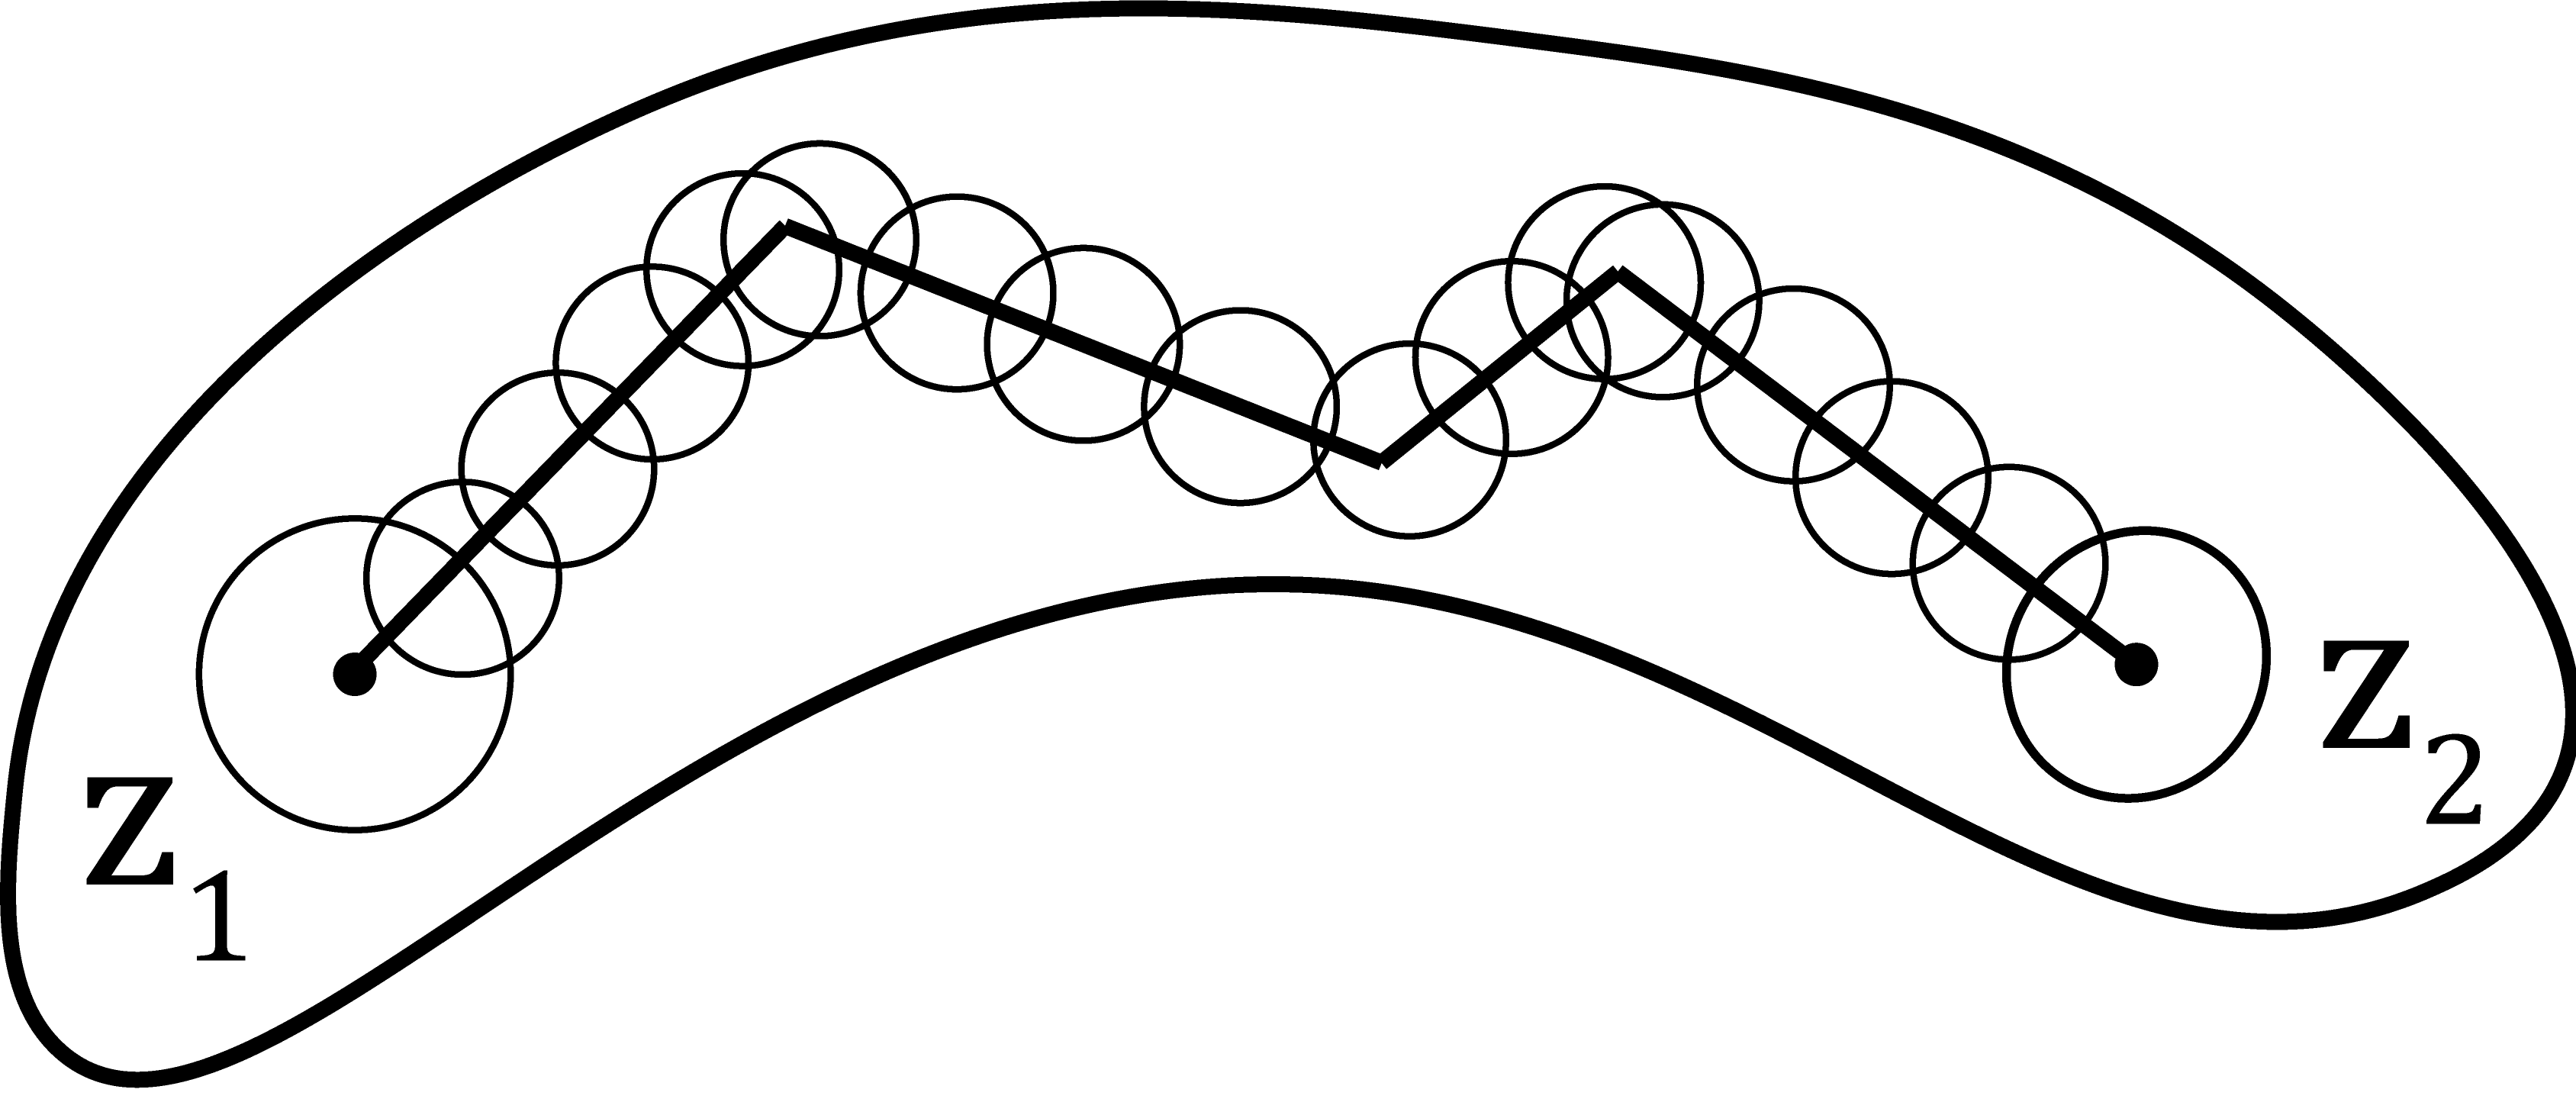
\includegraphics[width=5cm]{pics/9_8.png}
            \centering
        \end{figure}

		\[1) \q f'(z) = 0 = u'_x + i u'_y = v'_y + i v'_x\]
		\[\begin{cases}
				u'_x \equiv 0 \\
				u'_y \equiv 0 \\
				v'_x \equiv 0 \\
				v'_y \equiv 0
			\end{cases} \qq \forall (x, y) \in \Omega\]
		По лемме $f(z_2) = f(z_1) \q \forall z_1, z_2 \in \Omega$
		\[2) \q \real f = u(x, y) = const\]
		\[\Ra\begin{cases}
				\frac{\partial u}{\partial x} (x, y) = 0 \\
				\frac{\partial u}{\partial y} (x, y) = 0
			\end{cases} \forall (x, y) \in \Omega \Ra (\text{+ К-Р}) \begin{cases}
				\frac{\partial v}{\partial y} = 0 \\
				-\frac{\partial v}{\partial x} = 0
			\end{cases}\]
		По лемме $v = \const $ в $\Omega$ $\Ra f(z) = \const$
		\[3) \q \abs{f} = \const \Ra \abs{f}^2 = u^2 + v^2 = \const\]
		\[\begin{cases}
				2 u \cdot u'_x + 2v v_x' = 0 \\
				2 u \cdot u'_y + 2v v'_y = 0
			\end{cases} \q \begin{cases}
				u \cdot u'x - v \cdot u'_y = 0 \\
				u \cdot u'y + v \cdot u'_x = 0
			\end{cases}\]
		Определитель системы л. ур
		\[\begin{vmatrix}
				u & -v \\
				v & u
			\end{vmatrix} = y^2 + v^2 \neq 0\]
		Если $u^2 + v^2 \neq 0 \Ra u'_x = 0, u'_y = 0 \Ra u \equiv \const \Ra v \equiv \const$
		\[4) \q \text{arg } f(z) \equiv const \q \forall z \in \Omega\]
		\[\text{Введем функцию } k = \frac{u}{v} \Ra k = \const\]
		\[\text{Дифф. } \forall z \in \Omega \q (1 + ik)f = (1 + ik)(u + iv) = u + iku + iv - u\]
		\[\real ((1 + ik)f) = 0 \Ra (1 + ik)f \equiv \const\]
	\end{Proof}
\end{lect}
\end{document}
